First, we evaluate the segmentation quality of both models on the test set, reporting per‑class IoU and foreground mIoU over the head and tail classes.

\Cref{tab:segmentation_results} summarizes the results: ResUNet18 substantially outperforms UNet3 across all classes, achieving a foreground mIoU of \qty{0.71}{} compared to \qty{0.48}{} for UNet3.
ResUNet18 also achieves a notably lower segmentation loss and a higher background IoU.

\Cref{fig:segmentation_loss_curves} shows the training and validation loss curves over 10 epochs.
Both models converge quickly, but ResUNet18 starts to overfit after around four epochs, as indicated by an increase in validation loss.
Nevertheless, ResUNet18 consistently achieves lower losses than UNet3 throughout training -- UNet3 never reaches ResUNet18's loss levels, even at its best.

\Cref{fig:segmentation_predictions} presents qualitative predictions for three test samples for each model.
Each example shows the input image, the ground-truth mask and the predicted mask.
ResUNet18's predictions appear sharper and more accurate, with clear distinction between the head and tail, whereas UNet3's predictions are blurrier and more easily confused by noise from other bees or background clutter.

\begin{table}[htbp]
    \centering
    \caption{Segmentation performance on the test set.}
    \label{tab:segmentation_results}
    \begin{tabular}{lcccccc}
        \toprule
        \textbf{Model} & \textbf{\#Params} & \textbf{Test Loss} & \textbf{IoU$_{0}$} & \textbf{IoU$_{1}$} & \textbf{IoU$_{2}$} & \textbf{mIoU$_{1,2}$} \\
        \midrule
        UNet3          & \qty{1.93}{M}     & \qty{0.3620}{}     & \qty{0.8959}{}     & \qty{0.4852}{}     & \qty{0.4827}{}     & \qty{0.4839}{}        \\
        ResUNet18      & \qty{14.24}{M}    & \qty{0.1742}{}     & \qty{0.9482}{}     & \qty{0.7069}{}     & \qty{0.7205}{}    & \qty{0.7137}{}       \\
        \bottomrule
    \end{tabular}
\end{table}

\begin{figure}[htbp]
    \centering
    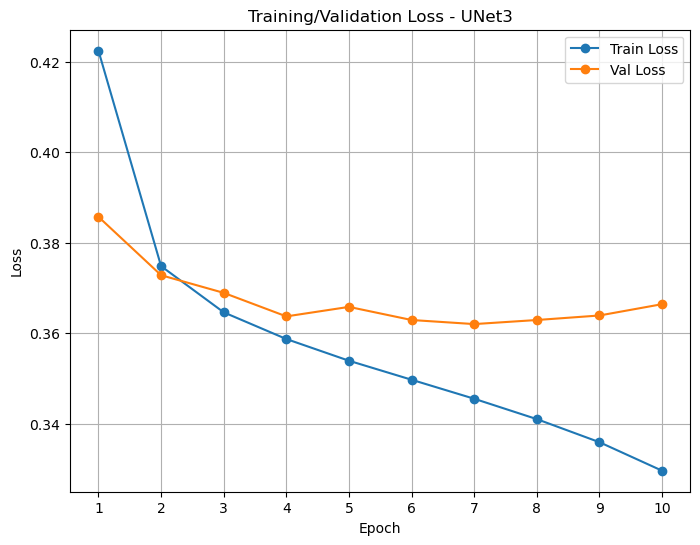
\includegraphics[width=0.49\textwidth]{figures/results/2 - segmentation performance/UNet3 Loss.png}
    \hfill
    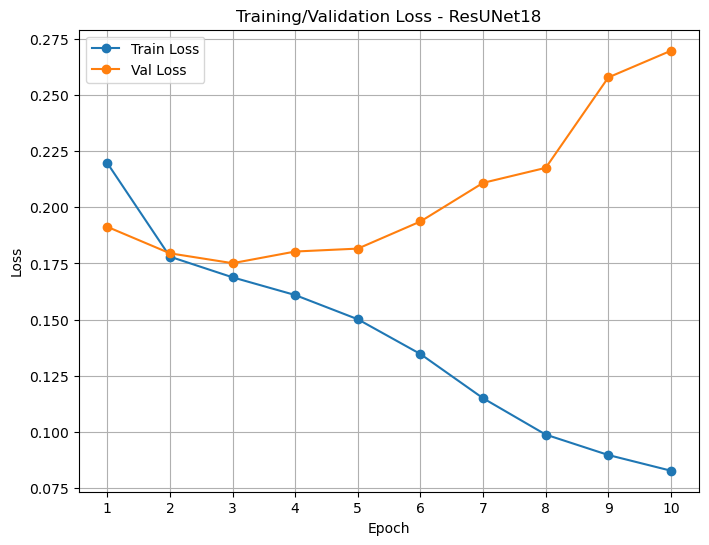
\includegraphics[width=0.49\textwidth]{figures/results/2 - segmentation performance/ResUNet18 Loss.png}
    \caption{
        Training and validation loss curves over 10 epochs for both models.
        (\textbf{Left}) UNet3 shows steady convergence but plateaus at a higher loss.
        (\textbf{Right}) ResUNet18 achieves lower training and validation loss overall but begins to overfit after about 4 epochs, as indicated by the upward trend in validation loss.
    }
    \label{fig:segmentation_loss_curves}
\end{figure}

\begin{figure}[htbp]
    \centering
    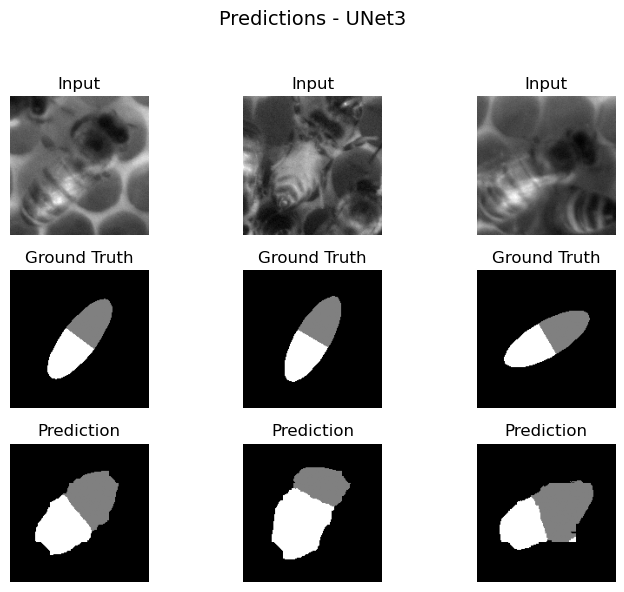
\includegraphics[width=0.49\textwidth]{figures/results/2 - segmentation performance/UNet3 Prediction Masks.png}
    \hfill
    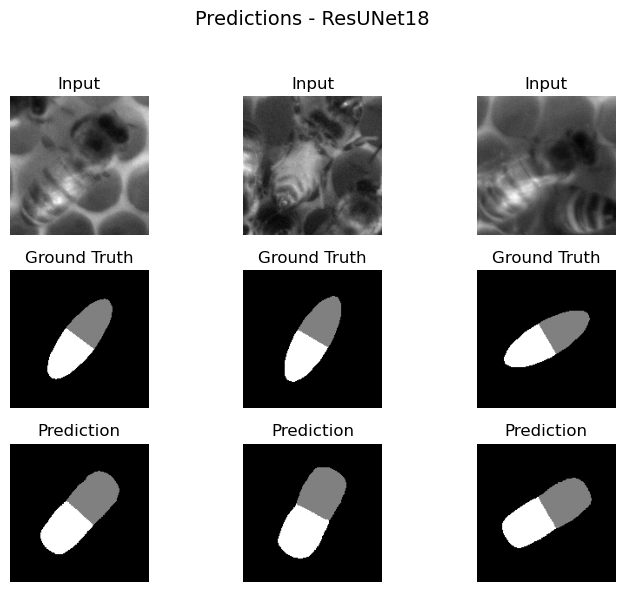
\includegraphics[width=0.49\textwidth]{figures/results/2 - segmentation performance/ResUNet18 Prediction Masks.png}
    \caption{
        Example segmentation predictions on three test samples for each model.
        Each column shows (\textit{top}) the input image, (\textit{middle}) the ground‑truth mask, and (\textit{bottom}) the predicted mask.
        (\textbf{Left}) UNet3 predictions are blurry and frequently misclassify head/tail regions due to noise and clutter.
        (\textbf{Right}) ResUNet18 predictions are sharper and better capture head and tail shapes, even in the presence of background bees and occlusions.
    }
    \label{fig:segmentation_predictions}
\end{figure}